%\documentclass{article}
\begin{comment}
\usepackage{tikz}
\usetikzlibrary{positioning}
\usetikzlibrary{shapes.geometric}
\usetikzlibrary{shapes.misc}
\usepackage{amsmath}
\usepackage{amssymb}
\usepackage{xstring}


\begin{document}
\end{comment}

\begin{figure}
\centering
\small 
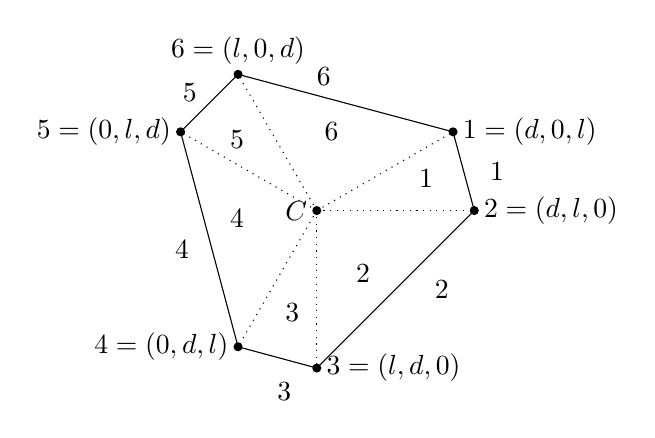
\begin{tikzpicture}

  \coordinate (A) at (1.73,1.00);
  \coordinate (B) at (-1,1.73);
  \coordinate (C) at (-1.73,1.00);
  \coordinate (D) at (-1,-1.73);
  \coordinate (E) at (0,-2);
  \coordinate (F) at (2,0);
  \coordinate (O) at (0,0);
  

\draw plot[tension=.7] coordinates { (1.73 ,1.00) (-1,1.73) (-1.73,1) (-1,-1.73) (0,-2) (2,0) (1.73,1) } ;
 
 
\draw [fill=black] (A) circle (0.05) node[below, right]{$\svi{1} =(d,0,l)$};
\draw [fill=black] (F) circle (0.05) node[right, black]{$\svi{2} =(d,l,0)$};
\draw [fill=black] (E) circle (0.05) node[right, black]{$\svi{3} = (l,d,0)$};

\draw [fill=black] (D) circle (0.05) node[left, black]{$\svi{4} =(0,d,l)$};
\draw [fill=black] (C) circle (0.05) node[left, black]{$\svi{5} = (0,l,d)$};
\draw [fill=black] (B) circle (0.05) node[above, black]{$\svi{6}=(l,0,d)$};

\draw [fill=black] (0,0) circle (0.05) node[left, black]{$C$};

\draw [dotted] (O) -- (A);
\draw [dotted] (O) -- (B);
\draw [dotted] (O) -- (C);
\draw [dotted] (O) -- (D);
\draw [dotted] (O) -- (E);
\draw [dotted] (O) -- (F);

\draw [fill=white] (2.5, .5) circle(0) node[left,black] {$\Fac{1}$};
\draw [fill=white] (1.8, -1) circle(0) node[left,black] {$\Fac{2}$};
\draw [fill=white] (-0.2, -2.3) circle(0) node[left,black] {$\Fac{3}$};
\draw [fill=white] (-1.5, -0.5) circle(0) node[left,black] {$\Fac{4}$};
\draw [fill=white] (-1.4, 1.5) circle(0) node[left,black] {$\Fac{5}$};
\draw [fill=white] (0.3, 1.7) circle(0) node[left,black] {$\Fac{6}$};



\draw [fill=white] (1.6, .4) circle(0) node[left,black] {$\Pyr{1}$};
\draw [fill=white] (.8, -.8) circle(0) node[left,black] {$\Pyr{2}$};
\draw [fill=white] (-.1, -1.3) circle(0) node[left,black] {$\Pyr{3}$};

\draw [fill=white] (-0.8, -0.1) circle(0) node[left,black] {$\Pyr{4}$};
\draw [fill=white] (-0.8, 0.9) circle(0) node[left,black] {$\Pyr{5}$};
\draw [fill=white] (.4, 1.) circle(0) node[left,black] {$\Pyr{6}$};


\end{tikzpicture}
\normalsize
\caption{Hexagonal $\favn$ for $Q = (s=1,n=2,\delta=0,\sat=0.6)$, with facets and pyramids labelled \cite{KumarTRO15}. Even-indexed pyramids are all congruent to each other, as are all odd-indexed ones.}
\label{fig:larged}
\end{figure}   

 %\end{tikzpicture}
%\end{document}